\section{Testing}

\subsection{Configuration}

\subsubsection{2048.h}
The first component included is the game logic, which resides in the file 
\textit{2048.h}. As \textit{2048.h} is a single-header library, the 
\texttt{\_2048\_IMPLEMENTATION} macro must be defined to ensure that the 
library includes the implementations of the game functions, rather than just 
their declarations.

After this, a declaration of the game table is made, which will store the 
state of the game. The direction enumeration type from \textit{2048.h} is 
extended to include the \textbf{flat} position and is renamed to 
\texttt{Orientation} accordingly.

\subsubsection{FastLED.h}
The next library included is \textit{FastLED.h}, which allows communication 
with the display. The \texttt{LED\_PIN} is configured and assigned to pin 
\texttt{32}; this can be changed to any other port as needed. The 
\texttt{LED\_BRIGHTNESS} ranges from \texttt{0-255}, and an arbitrary value 
of \texttt{16} has been chosen, but it can be adjusted as required. The 
\texttt{LED\_COUNT} is set to \texttt{64}, reflecting the number of LEDs in 
the display. Following this, the \texttt{leds} array is defined with a length 
matching \texttt{LED\_COUNT}.

\subsubsection{basicMPU6050.h}
The next library, \textit{basicMPU6050.h}, makes it easy to communicate 
with the MPU6050 sensor. An object named \texttt{mpu} is created to handle 
this interaction.

\subsubsection{Setup}
In the \texttt{setup} function, the random number generator (RNG) is 
initialized. The 2048 game table is set up with two tiles. 
The display and gyroscope are then configured.

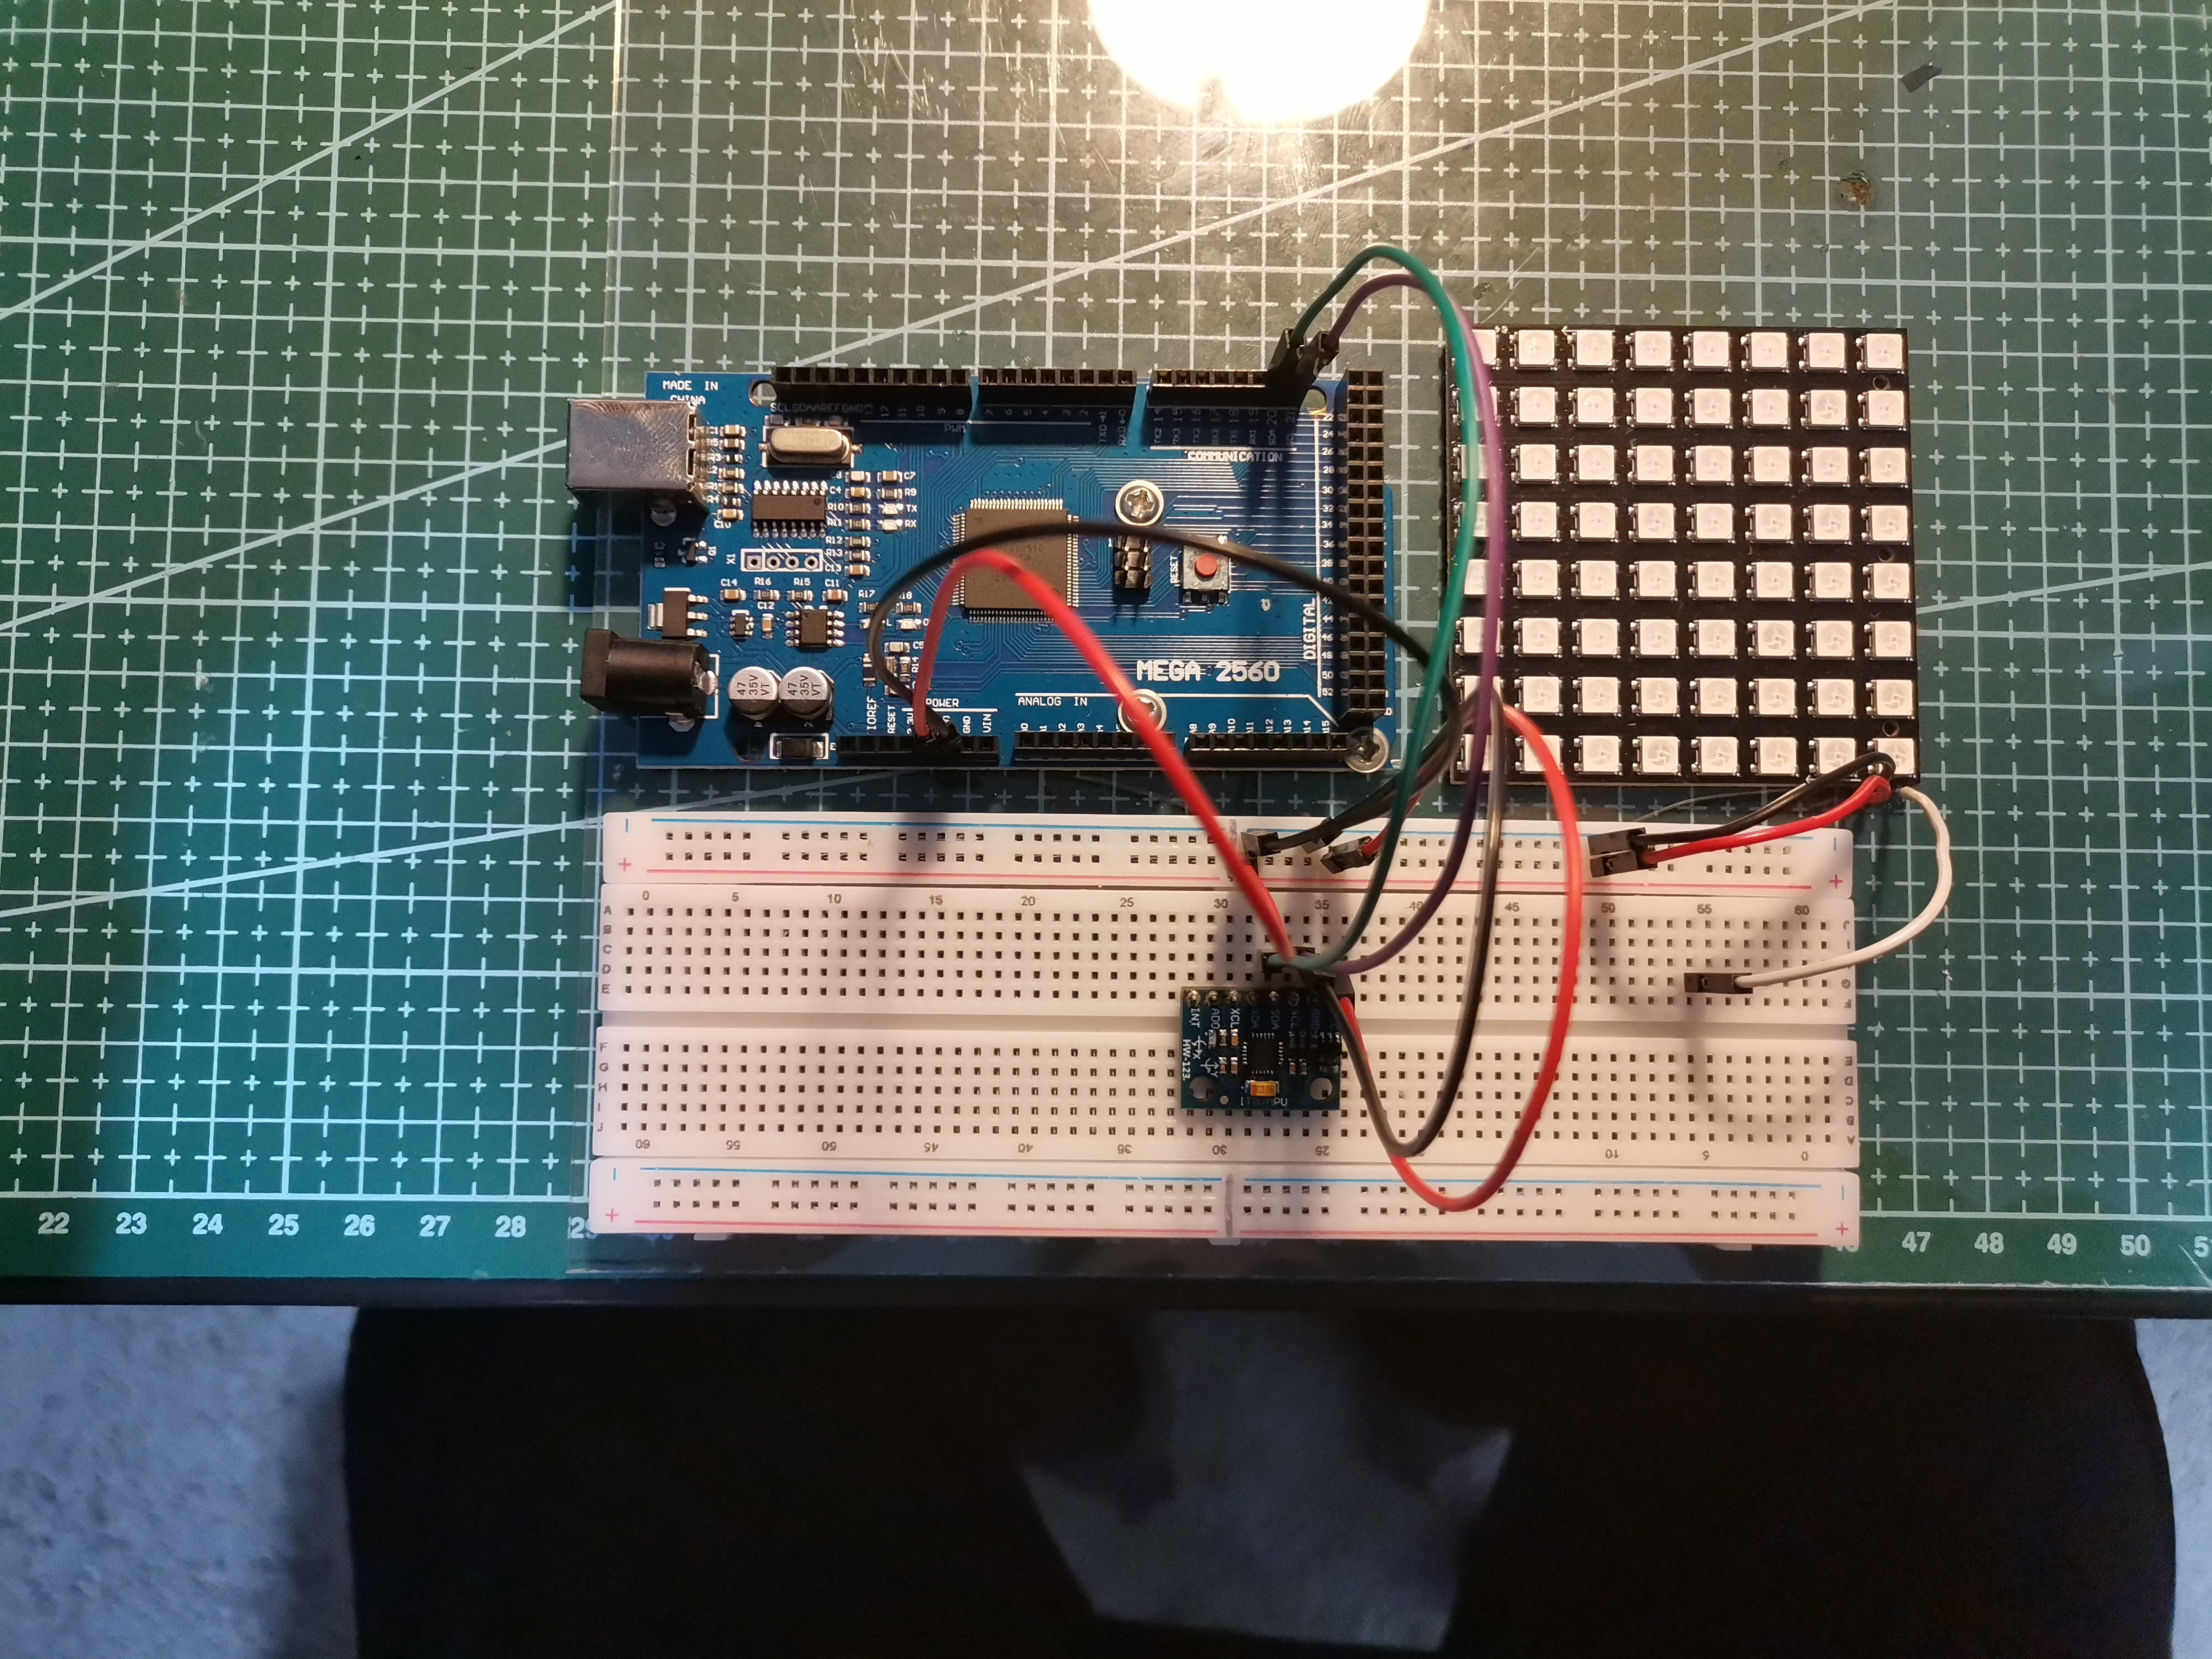
\includegraphics[width=1.0\linewidth]{demo/demo2.jpg}

\subsection{Logic}

\subsubsection{Display}
The \texttt{display()} function processes each row and column of the game 
table, calling the \texttt{draw\_cell()} function for each cell. 
Once completed, it calls \texttt{FastLED.show()} to refresh the display.
The \texttt{draw\_cell()} function assigns colors based on the current values 
in the game table to show on the display.
Additionally, a function named \texttt{cell\_color} is used to return a 
color based on the input number, using a predefined formula that can be 
adapted.

\subsubsection{Input}
The \texttt{getOrientation()} function retrieves inclination information from 
the accelerometer by calling the methods 
\texttt{mpu.ax()}, \texttt{mpu.ay()}, and \texttt{mpu.az()}.
It compares these values against a configurable \texttt{THRESHOLD}. 
The function utilizes two helper methods, \texttt{sup()} and \texttt{sub()}, 
which verify whether a value falls within the specified \texttt{THRESHOLD}.

\subsubsection{Loop}
The first action carried out by the \texttt{loop()} function is to display 
the current state of the game table. It then obtains the current 
orientation and compares it with the previous orientation. If a difference 
is found, the function determines the current orientation using a 
\texttt{switch} statement and calls the appropriate function from 
\texttt{2048.h}. Finally, it updates the \texttt{prev\_orientation} variable.
